% !TeX root = RJwrapper.tex
\title{User-Specified General-to-Specific and Indicator Saturation Methods}
\author{by Genaro Sucarrat}

\maketitle

\abstract{
General-to-Specific (GETS) modelling provides a comprehensive, systematic and cumulative approach to modelling that is ideally suited for conditional forecasting and counterfactual analysis, whereas Indicator Saturation (ISAT) is a powerful and flexible approach to the detection and estimation of structural breaks (e.g.\ changes in parameters), and to the detection of outliers. To these ends, multi-path backwards elimination, single and multiple hypothesis tests on the coefficients, diagnostics tests and goodness-of-fit measures are combined to produce a parsimonious final model. In many situations a specific model or estimator is needed, a specific set of diagnostics tests may be required, or a specific fit criterion is preferred. In these situations, if the combination of estimator/model, diagnostics tests and fit criterion is not offered in a pre-programmed way by publicly available software, then the implementation of user-specified GETS and ISAT methods puts a large programming-burden on the user. Generic functions and procedures that facilitate the implementation of user-specified GETS and ISAT methods for specific problems can therefore be of great benefit. The R package \pkg{gets} is the first software -- both inside and outside the R universe -- to provide a complete set of facilities for user-specified GETS and ISAT methods: User-specified model/estimator, user-specified diagnostics and user-specified goodness-of-fit criteria. The aim of this article is to illustrate how user-specified GETS and ISAT methods can be implemented with the R package \pkg{gets}. }

%%%%%% BOLD MATH-SYMBOLS:
\newcommand{\bx}{\boldsymbol{x}}
\newcommand{\bbeta}{\boldsymbol{\beta}}

\section{Introduction}

%Introductory section which may include references in parentheses \citep{R}, or cite a reference such as \citet{R} in the text.

General-to-Specific (GETS) modelling provides a comprehensive, systematic and cumulative approach to modelling that is ideally suited for scenario analysis, e.g.\ conditional forecasting and counterfactual analysis. To this end, well-known ingredients (tests of coefficients, multi-path backwards elimination, diagnostics tests and fit criteria) are combined to produce a parsimonious final model that passes the chosen diagnostics. GETS modelling originated at the London School of Economics (LSE) during the 1960s, and gained widespread acceptance and usage in economics during the 1980s and 1990s. The two-volume article collection by \citet{CamposEricssonHendry2005} provides a comprehensive historical overview of key-developments in GETS modelling. Software-wise, a milestone was reached in 1999, when the data-mining experiment of \citet{Lovell83} was re-visited by \citet{Hooveretal99}. They showed that automated GETS modelling could improve substantially upon the then prevalent modelling approaches. The study spurred numerous new studies and developments, including Indicator Saturation (ISAT) methods, see \citet{HendryJohansenSantos2008} and \citet{CastleDoornikHendryPretis2015}. ISAT methods provide a powerful and flexible approach to the detection and estimation of structural breaks (e.g.\ changes in parameters), and to the detection of outliers.

On CRAN, there are two packages that provide GETS methods. The second, named \CRANpkg{gets}, is simply the successor of the first, which is named \CRANpkg{AutoSEARCH}.\footnote{Both packages were created by me. Originally, I simply wanted to rename the first to the name of the second. This, however, is inconvenient in practice I was told, so I was instead asked by CRAN to publish a ``new" package with the new name.} Since October 2014 the development of \pkg{AutoSEARCH} is frozen, and all development efforts have been directed towards \pkg{gets} together with Dr.\ Felix Pretis and Dr.\ James Reade.\footnote{Recently, Jonas Kurle and Moritz Schwarz have also made contributions. See the Gitub page for the current development version of the package: \url{https://github.com/gsucarrat/gets/}.} An introduction to the \pkg{gets} package is provided by \cite{PretisReadeSucarrat2018}. However, it does does not cover the user-specification capabilities of the package, some of which were not available at the time.

At the time of writing (September 2020), the publicly available softwares that provide GETS and ISAT methods are contained in Table \ref{table:software:comparison}. Although they offer GETS and ISAT methods for some of the most popular models in applications, in many situations a specific model or estimator will be needed, a specific set of diagnostics tests may be required, or a specific fit criterion is preferred. In these situations, if the combination of estimator/model, diagnostics tests and fit criterion is not offered in a pre-programmed way by the publicly available softwares, then the implementation of user-specified GETS and ISAT methods puts a large programming-burden on the user. Generic functions and procedures that facilitate the implementation of user-specified GETS and ISAT methods for specific problems can therefore be of great benefit. The R package \pkg{gets}, since version 0.20 (September 2019), is the first software -- both inside and outside the R universe -- to provide a complete set of facilities for user-specified GETS and ISAT methods: User-specified model/estimator, user-specified diagnostics and user-specified goodness-of-fit criteria. The aim of this article is to illustrate how user-specified GETS and ISAT methods can be implemented.

\begin{table}[t!]
	\centering
	\setlength{\tabcolsep}{3pt} %needed to ensure table fits on page
	\begin{tabular}{lccccccc}
		\toprule
		& & $\underset{(\text{MATLAB})}{\text{HP1999}}$ &  $\underset{(\text{OxMetrics})}{\text{Autometrics}}$ & $\underset{(\text{Scilab})}{\text{Grocer}}$ & $\underset{(\text{STATA})}{ \text{genspec} }$ & EViews$^*$ & $\underset{(\text{R})}{ \text{ \pkg{gets} } }$ \\
		\midrule
		More than 10 paths & & & Yes & Yes & Yes & Yes & Yes \\[1mm] 
		GETS of linear regression & & Yes & Yes & Yes & Yes & Yes & Yes \\[1mm]
		GETS of variance models & & & & & & & Yes \\[1mm]
		GETS of logit/count models & & & Yes & & & & \\[1mm]
		GETS of probit models & & & Yes & Yes & & & \\[1mm]
		GETS of panel models & & & & Yes & Yes & & \\[1mm]
		GETS of MIDAS models & & & & & & Yes & \\[1mm]
		ISAT of linear regression & & & Yes & Yes & & Yes & Yes \\[1mm]
		User-specified GETS & &  &  & Yes & & & Yes \\[1mm]
		User-specified ISAT &  &  &  & & & & Yes \\[1mm]
		User-specified diagnostics &  & & & Yes & & & Yes \\[1mm]
		User-specified goodness-of-fit & & & & & & & Yes \\[1mm]
		Menu-based GUI &  & & Yes & & & Yes & \\[1mm]		
		Free and open source & & Yes$^{**}$ & & Yes & Yes$^{**}$ & & Yes \\[1mm]
		\bottomrule
	\end{tabular}\\
	\caption{
		\label{table:software:comparison}
		A comparison of publicly available GETS and ISAT softwares with emphasis on user-specification capabilities. HP1999, the MATLAB code of \citet{Hooveretal99}. Autometrics, OxMetrics version 15, see \citet{DoornikHendry2018}. Grocer, version 1.8, see \citet{DuboisMichaux2019}. genspec, version 1.2.2, see \citet{Clarke2014}. EViews, version 12, see \citet{EViews2020}. \pkg{gets}, version 0.25, see \cite{SucarratKurlePretisReadeSchwarz2020getsV025}, and \citet{PretisReadeSucarrat2018}.\\
		$^{*}$To be included in version 12 (November 2020).\\
		$^{**}$The modules in themselves are free and open source, but they run in non-free and closed source software environments (MATLAB and STATA, respectively).
	}
\end{table}

The rest of this article contains four sections. In the next section the model selection properties of GETS and ISAT methods are summarised. This is followed by a section that outlines the general principles of how user-specified estimation, user-specified diagnostics and user-specified goodness-of-fit measures are implemented. Next, a section with four illustrations follows. The final section contains a summary.

\section{Model selection properties of GETS and ISAT methods} 

It is useful to denote a generic model for observation $t$ as
%
\begin{equation}
	m\left(y_t, \bx_t, \bbeta \right), \qquad t=1,2,\ldots,n,
\end{equation}
%
where $y_t$ is the dependent variable, $\bx_t = (x_{1t}, x_{2t}, \ldots)'$ is a vector of covariates, $\bbeta = (\beta_1, \beta_2, \ldots)'$ is a vector of parameters to be estimated and $n$ is the sample size. Two examples are the linear regression model and the logit-model:
%
\begin{align}
	y_t &= \beta_1 x_{1t} + \cdots + \beta_k x_{kt} + \epsilon_t, \label{eq:linear:regression:model} \\
	Pr\left(y_t=1|\bx_t\right) &= \frac{1}{1+\exp\left(-h_t\right)} \qquad\text{with}\qquad h_t = \beta_1 x_{1t} + \cdots + \beta_k x_{kt}. \label{eq:linear:logit:model}
\end{align}
%
Note that, in a generic model $m(y_t, \bx_t, \bbeta)$, the dimension $\bbeta$ is usually -- but not necessarily -- equal to the dimension of $\bx_t$. Here, for notational convenience, they will both have dimension $k$ unless otherwise stated.

In \eqref{eq:linear:regression:model}--\eqref{eq:linear:logit:model}, a variable $x_{jt} \in \bx_t$ is said to be relevant if $\beta_j \neq 0$ and irrelevant if $\beta_j = 0$. Let $k_{\text{rel}} \geq 0$ and $k_{\text{irr}} \geq 0$ denote the number of relevant and irrelevant variables, respectively, such that $k_{\text{rel}} + k_{\text{irr}} = k$. GETS modelling aims at finding a specification that contains as many relevant variables as possible, and a proportion of irrelevant variables that on average equals the significance level $\alpha$ chosen by the investigator. Put differently, if $\widehat{k}_{\text{rel}}$ and $\widehat{k}_{\text{irr}}$ are the retained number of relevant and irrelevant variables in an empirical application, respectively, then GETS modelling aims at satisfying 
%
\begin{equation}\label{eq:asymptotic:gauge:and:potency}
	\E\left(\widehat{k}_{\text{rel}}/k_{\text{rel}}\right) \rightarrow 1 \quad \textnormal{and} \quad \E\left(\widehat{k}_{\text{irr}}/k_{\text{irr}}\right) \rightarrow \alpha \quad \textnormal{as} \quad n\rightarrow\infty,
\end{equation}
%
when $k_{\text{rel}},k_{\text{irr}}>0$.  If either $k_{\text{rel}}=0$ or $k_{\text{irr}}=0$, then the targets are modified in natural ways: If $k_{\text{rel}}=0$, then the first target is $\E\left(\widehat{k}_{\text{rel}}\right) = 0$, and if $k_{\text{irr}}=0$, then the second target is $\E\left(\widehat{k}_{\text{irr}}\right) = 0$. Sometimes, the irrelevance proportion $\widehat{k}_{\text{irr}}/k_{\text{irr}}$ is also referred to as \dfn{gauge}, whereas the relevance proportion $\widehat{k}_{\text{irr}}/k_{\text{irr}}$ is also referred to as \dfn{potency}.

In targeting a relevance proportion equal to 1 and an irrelevance proportion equal to $\alpha$, GETS modelling combines well-known ingredients: Multi-path backwards elimination, tests on the $\beta_j$'s (both single and multiple hypothesis tests), diagnostics tests and fit-measures (e.g. information criteria). Let $V\left(\widehat{\bbeta}\right)$ denote the estimated coefficient-covariance. GETS modelling in the package \pkg{gets} can be described as proceeding in three steps:\footnote{The way GETS modelling is implemented across softwares varies. For example, in Autometrics and Grocer the diagnostics are not checked at each deletion.} 

\begin{enumerate}
	\item Formulate a General Unrestricted Model (GUM), i.e.\ a starting model, that passes a set of chosen diagnostic tests. A regressor $x_j$ in the GUM is non-significant if the $p$-value of a two-sided $t$-test is lower than the chosen significance level $\alpha$, and each non-significant regressor constitutes the starting point of a backwards elimination path. The test-statistics of the $t$-tests are computed as $\widehat{\beta}_j/se\left(\widehat{\beta}_j\right)$, where $se\left(\widehat{\beta}_j\right)$ is the square root of the $j$th.\ element of the diagonal of $V\left(\widehat{\bbeta}\right)$.
	
	\item Undertake backwards elimination along multiple paths by removing, one-by-one, non-significant regressors as determined by the chosen significance level $\alpha$. Each removal is checked for validity against the chosen set of diagnostic tests, and for parsimonious encompassing (i.e.\ a multiple hypothesis test) against the GUM. These multiple hypothesis tests on subsets of $\bbeta$ are implemented as Wald-tests.
	
	\item Multi-path backwards elimination can result in multiple terminal models. The last step of GETS modelling consists of selecting, among the terminal models, the specification with the best fit according to a fit-criterion, e.g.\ the \cite{Schwarz1978} information criterion. 
\end{enumerate}

In ISAT methods, the vector $\bx_t$ contains at least $n-1$ indicators in addition to other covariates that are considered. Accordingly, standard estimation methods are infeasible, since the number of variables in $\bx_t$ is usually larger than the number of observations $n$. The solution to this problem provided by ISAT methods is to first organise $\bx_t$ into $B$ blocks: $\bx_t^{\left(1\right)}, \ldots, \bx_t^{\left(B\right)}$. These blocks need not be mutually exclusive, so a variable or subset of variables can appear in more than one block. Next, GETS modelling is applied to each block, which leads to $B$ final models. Note that, in the \code{isat} function, the default is that no diagnostic tests are undertaken. Finally, a new round of GETS modelling is undertaken with the union of the retained variables from the $B$ blocks as covariates in a new starting model (i.e.\ a new GUM). The model selection properties targeted by ISAT methods are the same as those of GETS methods. Note, however, that since the starting model (the GUM) contains at least $n-1$ regressors, a tiny significance level -- e.g.\ $\alpha=0.001$ or smaller -- is usually recommended in ISAT methods.

\section{User-specification: General principles} 

In the current version of the package \pkg{gets}, version 0.25, the functions that admit user-specified estimation are \code{arx}, \code{getsm}, \code{getsFun} and \code{isat}.\footnote{In the future, the plan is to also enable user-specified GETS modelling with the function \code{getsv}, which implements GETS modelling of the log-variance.} The user-specification principles are the same in all four. However, if the result (i.e.\ a list) returned from the user-specified estimator does not have the same structure as that returned from the default estimator \code{ols} (part of the \pkg{gets} package), then \code{arx}, \code{getsm} and \code{isat} may not always work as expected. This is particularly the case with respect to their extraction functions (e.g.\ \code{print}, \code{coef}, \code{residuals} and \code{predict}). User-specified diagnostics and goodness-of-fit functions are optional. By default, \code{getsFun} and \code{isat} do not perform any diagnostics tests, whereas the default in \code{arx} and \code{getsm} is to test the standardised residuals for autocorrelation and Autoregressive Heteroscedasticity (ARCH). This is implemented via the \code{diagnostics} function (part of the \pkg{gets} package). Also by default, all four functions use the \cite{Schwarz1978} information criterion as goodness-of-fit measure, which favours parsimony, via the \code{infocrit} function (part of the \pkg{gets} package).

\subsection{The getsFun function}

The recommended, most flexible and computationally most efficient approach to user-specified GETS modelling is via the \code{getsFun} function. Currently, it accepts up to twenty-five arguments. For the details of all these arguments, the reader is referred to the discussion of the \code{getsm} function (Section 5) in \cite{PretisReadeSucarrat2018}, and the help pages of \code{getsFun} (type \code{?getsFun}). For the purpose of user-specified estimation, user-specified diagnostics and user-specified goodness-of-fit measures, the most important arguments are:
%
\begin{example}
  getsFun(y, x,
    user.estimator = list(name = "ols"),
    user.diagnostics = NULL,
    gof.function = list(name = "infocrit", method = "sc"),
    gof.method = c("min", "max"),
    ...)
\end{example}
%
The \code{y} is the left-hand side variable (the regressand), \code{x} is the regressor or design matrix, \code{user.estimator} controls which estimator or model to use and further arguments -- if any -- to be passed on to the estimator, \code{user.diagnostics} controls the user-specified diagnostics if any, and \code{gof.function} and \code{gof.method} control the goodness-of-fit measure used. Note that \code{y} and \code{x} should satisfy \samp{is.vector(y) == TRUE} and \samp{is.matrix(x) == TRUE}, respectively, and enter in "clean" ways: If either \code{y} or \code{x} are objects of class, say, \code{"ts"} or \code{"zoo"}, then \code{getsFun} may not behave as expected. By default, the estimator \code{ols} is used with its default arguments, which implements OLS estimation via the \code{qr} function. The value \code{NULL} on \code{user.diagnostics} means no diagnostics checks are undertaken by default. The following code illustrates \code{getsFun} in linear regression (the default), and reproduces the information printed while searching:
%
\begin{example}
  n <- 40 #number of observations
  k <- 20 #number of Xs

  set.seed(123) #for reproducibility
  y <- rnorm(n) #generate Y
  x <- matrix(rnorm(n*k), n, k) #create matrix of Xs

  #do gets with default estimator (ols), store output in 'result':
  result <- getsFun(y, x)

  #the information printed while searching:
  18 path(s) to search
  Searching: 1 2 3 4 5 6 7 8 9 10 11 12 13 14 15 16 17 18 
\end{example}
%
The object named \code{result} is a list, and the code \code{summary(results)} returns a summary of its contents. The most important entries are:
%
\begin{itemize}
	\item \code{paths}: A list of vectors containing the searched paths. Each vector (i.e. path) indicates the sequence of deletion of the regressors. In the example above the first path is
	%
\begin{example}
  $paths[[1]]
  [1]  1 15  6  7  3 14 11 16  4  2  8 12  5  9 20 19 13
\end{example}

	That is, regressor no.\ 1 was the first to be deleted, regressor no.\ 15 was the second, regressor no.\ 6 was the third, and so on. If the regressors in \code{x} were named, then a name-representation of the first deletion path is obtained with \code{ colnames(x)[ paths[[1]] ]}.
	
	\item \code{terminals}: A list of vectors with the distinct terminal models of the specification search. In the example above it is equal to
	%
\begin{example}
  $terminals
  $terminals[[1]]
  [1] 10 17 18

  $terminals[[2]]
  [1] 10 18
\end{example}
	
	That is, two terminal models. The first contains regressors 10, 17 and 18, whereas the second contains regressors 10 and 18.
	
	\item \code{terminals.results}: A data frame with the goodness-of-fit information of the terminal models. In the above example the entry is equal to:
	%
\begin{example}
  $terminals.results
          info(sc)      logl  n k
  spec 1: 2.514707 -44.76081 40 3
  spec 2: 2.529923 -46.90958 40 2
\end{example}
	
	\code{spec 1} is short for specification 1, i.e.\ terminal model 1, and \code{spec 2} is short for specification 2, i.e.\ terminal model 2. \code{info(sc)} indicates that the \cite{Schwarz1978} criterion (the default) is used as goodness-of-fit measure, whereas \code{n} and \code{k} denote the number of observations and parameters, respectively. 
	
	\item \code{best.terminal}: An integer that indicates which terminal model is the best according to the goodness-of-fit criterion used. In the example above the value is 1.
	
	\item \code{specific.spec}: A vector of integers that indicates which regressors that are contained in the best terminal model. In the above example it is
\begin{example}
  $specific.spec
  [1] 10 17 18
\end{example}
	That is, the best terminal model contains regressors no.\ 10, 17 and 18.
\end{itemize} 

\subsection{User-specified estimation}

User-specified estimation is carried out via the \code{user.estimator} argument. By default, the argument is \code{NULL}, so no diagnostic tests are undertaken. To carry out diagnostics, the argument must be specified as a list containing at least one entry -- a character -- named \code{name} with the name of the estimator to be invoked.\footnote{To carry out the same diagnostics as the default of the \code{getsm} function, the argument can be set to \code{list(name = "diagnostics", pval = c(0.025, 0.025))}.} Optionally, the list can also contain an item named \code{envir}, a character, which indicates the environment in which the user-specified estimator resides. Additional entries in the list, if any, are passed on to the estimator as arguments.

The user-specified estimator must also satisfy the following:
%
\begin{enumerate}
	\item It should be of the form \code{myEstimator(y, x, ...)}, where \code{y} is a vector and \code{x} is a matrix. In other words, while the name of the function is arbitrary, the first argument should be the regressand and the second the matrix of covariates.
	
	\item The user-defined estimator should return a \code{list} with a minimum of six items:
	\begin{itemize}
		\item \code{n} (the number of observations)
		\item \code{k} (the number of coefficients)
		\item \code{df} (degrees of freedom, used in the $t$-tests)
		\item \code{coefficients} (a vector with the coefficient estimates)
		\item \code{vcov} (the coefficient covariance matrix)
		\item \code{logl} (a goodness-of-fit value, e.g.\ the log-likelihood)
	\end{itemize}
	%
	The items need not appear in this order. However, the naming should be exactly as indicated. If also the diagnostics and/or the goodness-of-fit criterion is user-specified, then additional objects may be required, see the subsections below on user-specified diagnostics and goodness-of-fit criteria. Note also that, if the goodness-of-fit criterion is user-specified, then \code{logl} can in certain situations be replaced by another item (which needs not be named \code{logl}). 
	
	\item The user-defined estimator must be able to handle \code{NULL} regressor-matrices, i.e.\ situations where either \code{NCOL(x)} is 0 or \code{is.null(x)} is \code{TRUE}. This is needed in situations where a terminal model is empty (i.e.\ no regressors are retained).
\end{enumerate}
%
To illustrate how the requirements above can be met in practice, suppose -- as an example -- that we would like to use the function \code{lm} for estimation rather than \code{ols}. The first step is then to make a function that calls \code{lm} while satisfying requirements 1 to 3:
%
\begin{example}
  lmFun <- function(y, x, ...){

    ##create list:
    result <- list()

    ##n, k and df:
    result$n <- length(y)
    if( is.null(x) || NCOL(x) == 0 ){
      result$k <- 0
    }else{
      result$k <- NCOL(x)
    }
    result$df <- result$n - result$k

    ##call lm if k > 0:
    if( result$k > 0){
      tmp <- lm(y ~ x - 1)
      result$coefficients <- coef(tmp)
      result$vcov <- vcov(tmp)
      result$logl <- as.numeric(logLik(tmp))
    }else{
      result$coefficients <- NULL 
      result$vcov <- NULL
      result$logl <- sum(dnorm(y, sd = sqrt(var(y)), log = TRUE))
    }  

    ##return result: 
    return(result)

  }
\end{example}
%
The code
%
\begin{example}
  getsFun(y, x, user.estimator = list(name = "lmFun"))
\end{example}
%
undertakes the same specification search as earlier, but uses \code{lmFun} rather than \code{ols}.

\subsection{User-specified diagnostics}

User-specified diagnostics is carried out via the \code{user.diagnostics} argument. The argument must be a list containing at least two entries: A character named \code{name} containing the name of the diagnostics function to be called, and an entry named \code{pval} that contains a vector with values between 0 and 1, i.e.\ the chosen significance level(s) for the diagnostics test(s).\footnote{A word of caution is required. Let $R^{\left(i\right)}$ denote the event of rejecting the null, under the null, for a significance level $\alpha^{\left(i\right)}$ in diagnostic test $i$. For example, if only a single test is undertaken so that $i=1$, then $Pr(R^{\left(1\right)}) = \alpha^{\left(1\right)}$. If two tests are undertaken, however, then the probability of rejecting in one or both tests is $Pr\left(R^{\left(1\right)} \cup R^{\left(2\right)}\right)$. As rule of thumb, therefore, to control the overall error, it is recommended that the significance level of each diagnostic test is set equal to $\alpha/m$, where $\alpha$ is the overall or total significance level targeted by the user, and $m$ is the number of diagnostic tests. This is sometimes referred to as a Bonferroni correction.} If only a single test is undertaken by the diagnostics function, then \code{pval} should be of length one. If two tests are undertaken, then \code{pval} should be of length two. And so on. An example of the argument when only a single test is undertaken is:
%
\begin{example}
  user.diagnostics = list(name = "myDiagnostics", pval = 0.05))
\end{example}
%
That is, the name of the function is \code{myDiagnostics}, and the chosen significance level for the single test that is carried out is 5\%. Optionally, just as when the estimator is user-specified, the list can contain an item named \code{envir}, a character, which indicates the environment in which the user-specified diagnostics function resides. Additional items in the list, if any, are passed on to the user-specified function as arguments.

The user-specified diagnostics function must satisfy the following:
%
\begin{enumerate}
	\item It should be of the form \code{myDiagnostics(result, ...)}, where \code{result} is the list returned from the estimator in question, e.g.\ that of the user-specified estimator (recall requirement 2 in the previous section above).
	
	\item It should return an $m \times 3$ matrix that contains the $p$-value(s) of the test(s) in the third column, where $m\geq 1$ is the number of tests carried out. So if only a single test is carried out, then $m=1$ and the $p$-value should be contained in the third column. An example could look like:
	%
\begin{example}
            statistic df   pval
  normality        NA NA 0.0734
\end{example}
	%
	Note that the row-names and column-names in the example are not required. However, they do indicate what kind of information you may wish to put there for reporting purposes, e.g.\ by using the function \code{diagnostics} (also part of the \pkg{gets} package).
\end{enumerate}
%
To illustrate how the requirements can be met in practice, suppose we would like to ensure the residuals are normal by testing for non-normality with the Shapiro-Wilks test function \code{shapiro.test}. In this context, its main argument is the residuals of the estimated model. The list returned by the user-defined estimator named \code{lmFun} above, however, does not contain an item with the residuals. The first step, therefore, is to modify the estimator \code{lmFun} so that the returned list also contains the residuals:
%
\begin{example}
  lmFun <- function(y, x, ...){

    ##info needed for estimation:
    result <- list()
    result$n <- length(y)
    if( is.null(x) || NCOL(x)==0 ){
      result$k <- 0
    }else{
      result$k <- NCOL(x)
    }
    result$df <- result$n - result$k
    if( result$k > 0){
      tmp <- lm(y ~ x - 1)
      result$coefficients <- coef(tmp)
      result$vcov <- vcov(tmp)
      result$logl <- as.numeric(logLik(tmp))
    }else{
      result$coefficients <- NULL
      result$vcov <- NULL
      result$logl <- sum(dnorm(y, sd=sqrt(var(y)), log=TRUE))
    }   

    ##residuals:
    if( result$k > 0){
      result$residuals <- residuals(tmp)
    }else{
      result$residuals <- y
    }

    return(result)
  }
\end{example}
%
Computationally, the only modification appears under \verb|##residuals|. We can now make the user-specified diagnostics function:
%
\begin{example}
  myDiagnostics <- function(x, ...){
    tmp <- shapiro.test(x$residuals) #do the test
    result <- rbind( c(tmp$statistic, NA, tmp$p.value) )
    return(result)
  }
\end{example}
%
The following code undertakes GETS modelling with the user-specified estimator defined above, and the user-specified diagnostics function using a 5\% significance level for the latter:
%
\begin{example}
  getsFun(y, x, user.estimator = list(name = "lmFun"),
    user.diagnostics = list(name = "myDiagnostics", pval = 0.05))
\end{example}
%
Note that if the chosen significance level for the diagnostics is sufficiently high, then no specification search is undertaken because the starting model does not pass the non-normality test. With the current data, for example, a little bit of trial and error reveals this is the case for a level of about \code{pval = 0.35}.

\subsection{User-specified goodness-of-fit}

User-specified goodness-of-fit is carried out with the \code{gof.function} and \code{gof.method} arguments. The former indicates which Goodness-of-Fit (GOF) function to use, and the second is a character that indicates whether the best model maximises (\code{"max"}) or minimises (\code{"min"}) the GOF criterion in question. The first argument is a list with a structure similar to earlier: It must contain at least one entry, a character named \code{name}, with the name of the GOF function to call. An example is:
%
\begin{example}
  gof.function = list(name = "myGof"))
\end{example}
%
Optionally, also here the list can contain an item named \code{envir}, a character, which indicates the environment in which the user-specified GOF function resides. Also as earlier, additional items in the list are passed on to the user-specified GOF function as arguments. The default value, for example, \code{gof.function = list(name = "infocrit", method = "sc")}, means the argument \code{method = "sc"} is passed on to the function \code{infocrit}, see the help pages of \code{infocrit} (type \code{?infocrit}) for information on the methods available via this function. The user-specified GOF function must satisfy the following:
%
\begin{enumerate}
	\item It should be of the form \code{myGof(result, ...)}, where \code{result} is the list returned from the estimator in question, e.g.\ that of the user-specified estimator.
	
	\item It should return a single numeric value, i.e.\ the value of the GOF measure in question. 
\end{enumerate}
%
To illustrate how the requirements can be met in practice, suppose we would like to use the adjusted $R^2$ as our GOF measure in combination with our user-defined estimator. For the moment, the user-defined estimator \code{lmFun} does not contain the information necessary to compute the adjusted $R^2$. In particular, it lacks the regressand \code{y}. However, this is readily added:
%
\begin{example}
  lmFun <- function(y, x, ...){

    ##info needed for estimation:
    result <- list()
    result$n <- length(y)
    if( is.null(x) || NCOL(x)==0 ){
      result$k <- 0
    }else{
      result$k <- NCOL(x)
    }
    result$df <- result$n - result$k
    if( result$k > 0){
      tmp <- lm(y ~ x - 1)
      result$coefficients <- coef(tmp)
      result$vcov <- vcov(tmp)
      result$logl <- as.numeric(logLik(tmp))
    }else{
      result$coefficients <- NULL
      result$vcov <- NULL
      result$logl <- sum(dnorm(y, sd=sqrt(var(y)), log=TRUE))
    }  

    ##residuals:
    if( result$k > 0){
      result$residuals <- residuals(tmp)
    }else{
      result$residuals <- y
    }

    ##info needed for r-squared:
    result$y <- y

    return(result)
  }
\end{example}
%
The added part appears under \verb|##info needed for r-squared|. A GOF function that returns the adjusted $R^2$ is:
%
\begin{example}
  myGof <- function(object, ...){
    TSS <- sum((object$y - mean(object$y))^2)
    RSS <- sum(object$residuals^2)
    Rsquared <- 1 - RSS/TSS
    result <- 1 - (1 - Rsquared) * (object$n - 1)/(object$n - object$k)
    return(result)
  }
\end{example}
%
The following code undertakes GETS modelling with all the three user-specified functions defined so far:
%
\begin{example}
  getsFun(y, x, user.estimator = list(name = "lmFun"),
    user.diagnostics = list(name = "myDiagnostics", pval = 0.05),
    gof.function = list(name = "myGof"), gof.method = "max")
\end{example}
%
Incidentally, it leads to the same final model as when the default GOF function is used.

\subsection{More speed: turbo, max.paths, parallel computing}

In multi-path backwards elimination search, one may frequently arrive at a specification that has already been estimated and tested. As an example, consider the following two paths:
%
\begin{example}
  $paths[[1]]
  [1]  2 4 3 1 5

  $paths[[2]]
  [1]  4 2 3 1 5
\end{example}
%
In path 1, i.e.\ \code{paths[[1]]}, regressor no.\ 2 is the first to be deleted, regressor no.\ 4 is the second, and so on. In path 2 regressor no.\ 4 is the first to be deleted, regressor no.\ 2 is the second, and so on. In other words, after the deletion of the first two variables, the set of remaining variables (i.e.\ 3, 1 and 5) in the two paths is identical. Accordingly, knowing the result from the first path, in path 2 it is unnecessary to proceed further after having deleted the first two regressors. Setting the argument \code{turbo} equal to \code{TRUE} turns such a check on, and thus skips searches, estimations and tests that are unnecessary. The turbo comes at a small computational cost (often less than 1 second), since the check is undertaken at each deletion. This is why the default is \code{turbo = FALSE}. However, if the estimation time is noticeable, then turning the turbo on can reduce the search time substantially. As a rule of thumb, if each estimation takes 1 second or more, then turning the turbo on will (almost) always reduce the total search time.

Searching more paths may increase the relevance proportion or potency. Whether and to what extent this happens depends on the sample size $n$, and on the degree of multicolinearity among the regressors $\bx_t$. If $n$ is sufficiently large, or if the regressors are sufficiently uncorrelated, then searching fewer paths will not reduce the relevance proportion. In many situations, therefore, one may consider reducing the number of paths to increase the speed. This is achieved via the \code{max.paths} argument. Setting \code{max.paths = 10}, for example, means a maximum of 10 paths is searched. The paths that are searched are those of the 10 most insignificant variables (i.e.\ those with the highest $p$-values) in the starting model.

When implementing ISAT methods, the function \code{isat} undertakes a multi-round form of GETS modelling. In the first round the variables are split into $B$ blocks, and then GETS modelling is undertaken on each block. This is a socalled "embarassingly parallel" problem. To make \code{isat} search in parallel during the first round, simply set the argument \code{parallel.options} equal to an integer greater than 1. The integer determines how many cores/threads to use, and the command \code{detectCores()} can be used to find out how many cores/threads that are available on the current machine. Remember, it is not recommended to use all the cores/threads available. Within \code{isat}, parallel-computing is implemented with the \code{makeCluster} and \code{parApply} functions from the package \pkg{parallel}. If the time required by \code{makeCluster} to set up parallel computing is negligible relative to the total computing time (on an average computer the setup-time is about 1 second), then the total computing time may -- in optimal situations -- be reduced by a factor of about $m-0.8$, where $m>1$ is the number of cores/threads used for parallel computing.

\section{User-specified GETS and ISAT methods: Illustrations}

\subsection{GETS modelling of Generalised Linear Models (GLMs)}

The function \code{glm} enables the estimation of a large number of specifications within the class of Generalised Linear Models (GLMs). Here, it is illustrated how GETS modelling can be implemented with GLMs. To fix ideas, the illustration is in terms of the logit-model.

Let $y_t \in \left\{0,1\right\}$ denote the regressand of the logit-model given by
%
\begin{equation}
	Pr\left(y_t=1|\bx_t\right) = \frac{1}{1+\exp\left(-h_t\right)}, \qquad h_t = \bbeta'\bx_t.
\end{equation}
%
Next, consider the following set of data:
%
\begin{example}
  n <- 40 #number of observations
  k <- 20 #number of Xs
  set.seed(123) #for reproducibility
  y <- round(runif(40)) #generate Y
  x <- matrix(rnorm(n*k), n, k) #create matrix of Xs
\end{example}
%
In other words, one regressand $y_t \in \left\{0,1\right\}$ which is entirely independent of the 20 regressors in $\bx_t$. The following function enables GETS modelling of logit-models:

\begin{example}
  logitFun <- function(y, x, ...){

    ##create list:
    result <- list()

    ##n, k and df:
    result$n <- length(y)
    if( is.null(x) || NCOL(x)==0 ){
      result$k <- 0
    }else{
      result$k <- NCOL(x)
    }
    result$df <- result$n - result$k

    ##call glm if k > 0:
    if( result$k > 0){
      tmp <- glm(y ~ x - 1, family = binomial(link="logit"))
      result$coefficients <- coef(tmp)
      result$vcov <- vcov(tmp)
      result$logl <- as.numeric(logLik(tmp))
    }else{
      result$coefficients <- NULL
      result$vcov <- NULL
      result$logl <- result$n*log(0.5)
    }  

    ##return result:
    return(result)
  }
\end{example} 
%
To undertake the GETS modelling:
%
\begin{example}
  getsFun(y, x, user.estimator=list(name="logitFun"))
\end{example}
%
Two variables are retained, namely $x_{5t}$ and $x_{11t}$, at the default significance level of 5\% (i.e.\ \code{t.pval = 0.05}). To reduce the chance of retaining irrelevant variables, the significance level can be lowered to, say, 1\% by setting \code{t.pval = 0.01}.

To implement GETS modelling for a different GLM model, only two lines of code needs to be modified in the user-defined function above. The first is the line that specifies the \code{family}, and the second is the one that contains the log-likelihood associated with the empty model (i.e.\ the line \samp{result\$logl <- result\$n*log(0.5)}).

\subsection{Creating a \code{gets} method (S3) for the \code{"lm"} class of models}

The package \pkg{gets} provides the generic function \code{gets}. This enables the creation of GETS methods (S3) for models of arbitrary classes (type \code{?S3Methods} for more info on S3 methods). Here, this is illustrated for models of class \code{"lm"}. Our aim is to be able to do the following:
%
\begin{example}
	mymodel <- lm(y ~ x)
	gets(mymodel)
\end{example}
%
That is, to first estimate a model of class \code{"lm"} where \code{x} is a matrix of regressors, and then to conveniently undertake GETS modelling by simply applying the code \code{gets(.)} to the named object \code{mymodel}. To this end, a function named \code{gets.lm} that relies on \code{getsFun} will be created. In doing so, a practical aspect is how to appropriately deal with the intercept codewise. Indeed, as we will see, a notable part of the code in the user-defined function will be devoted to the intercept. The reason for this is that \code{lm} includes the intercept by default. Another practical aspect is whether to use \code{lm} or \code{ols} whenever a model is estimated by OLS (both employ the QR decomposition). The latter is simpler codewise and computationally faster, so we opt for the latter. The function is:
%
\begin{example}
  gets.lm <- function(object, ...){

    ##make y:
    y <- as.vector(object$model[, 1])
    yName <- names(object$model)[1]

    ##make x:
    x <- as.matrix(object$model[, -1])
    xNames <- colnames(x)
    if(NCOL(x) == 0){
      x <- NULL
      xNames <- NULL
    }else{
      if(is.null(xNames)){
        xNames <- paste0("X", 1:NCOL(x))
        colnames(x) <- xNames
      }
    }

    ##is there an intercept?:
    if(length(coef(object)) > 0){
      cTRUE <- names(coef(object))[1] == "(Intercept)"
      if(cTRUE){
        x <- cbind(rep(1, NROW(y)), x)
        xNames <- c("(Intercept)", xNames)
        colnames(x) <- xNames
      }
    }

    ##do gets:
    myspecific <- getsFun(y, x, ...)

    ##which are the retained regressors?:
    retainedXs <- xNames[myspecific$specific.spec]
    cat("Retained regressors:\n ", retainedXs, "\n")

    ##return result
    return(myspecific)

  }
\end{example}
%
Next, recall the Data Generation Process (DGP) of the first experiment:
%
\begin{example}
  n <- 40 #number of observations
  k <- 20 #number of Xs
  set.seed(123) #for reproducibility
  y <- rnorm(n) #generate Y
  x <- matrix(rnorm(n*k), n, k) #create matrix of Xs
\end{example}
%
We can now do GETS modelling on models of class \code{"lm"} by simply applying the code \samp{gets(...)} on the object in question. The following code first stores an estimated model of class \code{"lm"} in an object named \code{startmodel}, and then applies the newly defined function \code{gets.lm} to it:
%
\begin{example}
  startmodel <- lm(y ~ x)
  finallm <- gets(startmodel)	
\end{example}
%
The information from the specification search is stored in the object called \code{finallm}, and during the search the following is printed:
%
\begin{example}
  18 path(s) to search
  Searching: 1 2 3 4 5 6 7 8 9 10 11 12 13 14 15 16 17 18 
  Retained regressors:
  X10 X17 X18
\end{example}
%
In other words, the retained regressors are no.\ 10, 17 and 18. Note that, due to the way the user-defined function has been put together, the intercept is excluded from deletion.

\subsection{Regression with ARMA error}

The function \code{arima} can be used to estimate a linear regression with deterministic regressors and an error-term that follows an ARMA. An example is
%
\begin{equation*}
	y_t = \bbeta'\bx_{t} + \epsilon_t, \qquad \epsilon_t = \phi_1\epsilon_{t-1} + \theta_1 u_{t-1} + u_t, \qquad u_t\sim WN\left(0,\sigma_u^2\right),
\end{equation*} 
%
where $\bx_t$ is a vector of deterministic regressors and $WN$ is short for White Noise. The error $\epsilon_t$ is thus governed by an ARMA(1,1). Let $x_t$ denote a (deterministic) step-shift variable in which the step-shift occurs at observation 30, i.e.\ $x_t = 1\left(t\geq30\right)$. Next, consider the DGP given by
%
\begin{equation}\label{eq:dgp:of:location-shift}
	y_t = 4x_t + \epsilon_t, \qquad \epsilon_t = 0.4\epsilon_{t-1} + 0.1 u_{t-1} + u_t, \qquad u_t \sim N\left(0,1\right), \qquad t=1,\ldots,n
\end{equation}
%
with $n=60$. In other words, the series $y_t$ is non-stationary and characterised by a large location shift at $t=30$. Figure \ref{figure:step-shift} illustrates the evolution of $y_t$, which is generated with the following code:
%
\begin{example}
  set.seed(123) #for reproducibility
  eps <- arima.sim(list(ar = 0.4, ma = 0.1), 60) #epsilon
  x <- coredata(sim(eps, which.ones = 30)) #step-dummy at t = 30
  y <- 4*x + eps #the dgp
  plot(y, ylab="y", xlab="t", lwd = 2)
\end{example}
%
\begin{figure}[htbp]
	\centering
	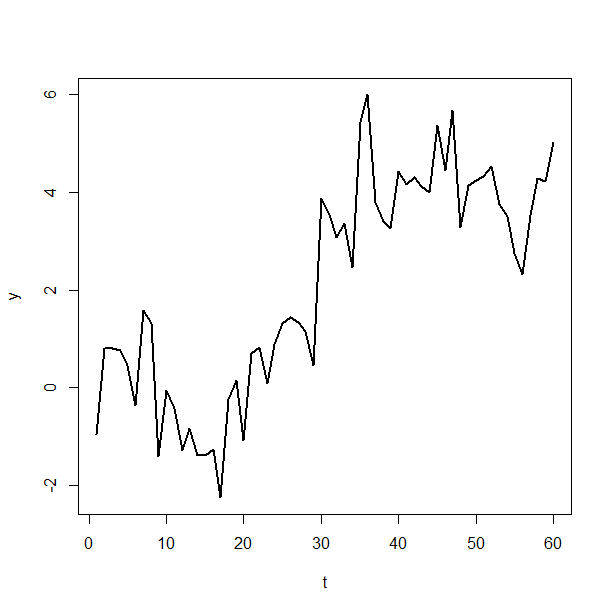
\includegraphics[scale=0.5]{step-shift}
	\caption{The graph of $y_t$ as given in \eqref{eq:dgp:of:location-shift}.}
	\label{figure:step-shift}
\end{figure}
%
By just looking at the graph, it seems clear that there is a location shift, but it is not so clear that it in fact occurs at $t=30$. I now illustrate how the \code{arima} function can be used in combination with \code{getsFun} to automatically search for where the break occurs. The idea is to do GETS modelling over a set or block of step-indicators that cover the period in which the break visually appears to be in. Specifically, the aim is to apply GETS modelling to the following starting model with 11 regressors:
%
\begin{equation*}
	y_t = \sum_{i=1}^{11} \beta_i \cdot 1_{ \left\{ t \geq 24+i \right\} } + \epsilon_t, \qquad \epsilon_t = \phi_1 \epsilon_{t-1} + \theta_1 u_{t-1} + u_t.
\end{equation*} 
%
To this end, we first need to make the user-specified estimator:
%
\begin{example}
  myEstimator <- function(y, x){

    ##create list:
    result <- list()

    ##estimate model:
    if( is.null(x) || NCOL(x)==0 ){
      result$k <- 0
      tmp <- arima(y, order = c(1,0,1)) #empty model
    }else{
      result$k <- NCOL(x)
      tmp <- arima(y, order = c(1,0,1), xreg = x)
      result$coefficients <- tmp$coef[-c(1:3)]
      result$vcov <- tmp$var.coef
      result$vcov <- result$vcov[-c(1:3),-c(1:3)]
    }

    ##rename and re-organise things:
    result$n <- tmp$nobs
    result$df <- result$n - result$k
    result$logl <- tmp$loglik

    return(result)
  }
\end{example}
%
Note that the estimator has been put together such that the ARMA(1,1) specification of the error $\epsilon_t$ is fixed. As a consequence, the specification search is only over the regressors. The following code first creates the 11 step dummies, and then undertakes the GETS modelling:
%
\begin{example}
  xregs <- coredata(sim(eps, which.ones = 25:35)) #11 step-dummies
  getsFun(y, xregs, user.estimator = list(name = "myEstimator"))
\end{example}
%
Two step-dummies are retained, namely those of $t=30$ and $t=35$.

\subsection{Faster ISAT when $n$ is large}

ISAT methods are computationally intensive, since at least $n-1$ indicators are included as regressors. Accordingly, as $n$ grows large, purpose-specific estimators can greatly reduce the computing time. One way of building such an estimator is by using tools from the package \CRANpkg{Matrix}, see \citet{BatesMaechler2018}. The code below illustrates this. First it loads the library, and then it creates a function named \code{olsFaster} that re-produces the structure of the estimation result returned by the function \code{ols} with \code{method = 3} (i.e.\ OLS with the ordinary coefficient-covariance), but with functions from \pkg{Matrix}. The code is: 
%
\begin{example}
  library(Matrix)
  olsFaster <- function(y, x){
    out <- list()
    out$n <- length(y)
    if (is.null(x)){ out$k <- 0 }else{ out$k <- NCOL(x) }
      out$df <- out$n - out$k
      if (out$k > 0) {
        x <- as(x, "dgeMatrix")
        out$xpy <- crossprod(x, y)
        out$xtx <- crossprod(x)
        out$coefficients <- as.numeric(solve(out$xtx,out$xpy))
        out$xtxinv <- solve(out$xtx)
        out$fit <- out$fit <- as.vector(x %*% out$coefficients)  
    }else{ out$fit <- rep(0, out$n)	}
    out$residuals <- y - out$fit
    out$residuals2 <- out$residuals^2
    out$rss <- sum(out$residuals2)
    out$sigma2 <- out$rss/out$df
    if (out$k > 0) { out$vcov <- as.matrix(out$sigma2 * out$xtxinv) }
    out$logl <- -out$n * log(2 * out$sigma2 * pi)/2 - out$rss/(2 * out$sigma2)
    return(out)            
  }
\end{example}
%
Depending on the data and hardware/software configuration, the estimator may lead to a considerably speed-improvement. In the following example, the function \code{system.time} suggests a speed improvement of about 20\% on the current hardware/software configuration: 
%
\begin{example}
  set.seed(123) #for reproducibility
  y <- rnorm(1000)
  x <- matrix(rnorm(length(y)*20), length(y), 20)
  #with ols:
  system.time( finalmodel <- isat(y, mxreg = x, max.paths = 5))
  #with olsFaster:
  system.time( finalmodel <- isat(y, mxreg = x, max.paths = 5,
    user.estimator = list(name = "olsFaster")) )
\end{example}

\section{Summary}

In many applications a specific model or estimator is needed, a specific set of diagnostics tests may be required, or a specific fit criterion is preferred. In these situations, if the combination of estimator/model, diagnostics tests and fit criterion is not already offered in a pre-programmed way by publicly available software, the implementation of user-specified GETS and ISAT methods puts a large programming-burden on the user. This article has outlined how recent additions to the package \pkg{gets} greatly simplifies the development of user-specified GETS and ISAT methods. The package is the first software -- both inside and outside the R universe -- to provide a complete set of facilities for user-specified GETS and ISAT methods.

\section{Acknowledgements}

I am grateful to the Editor Catherine Hurley, an anonymous reviewer, Damian Clarke, {\'E}ric Dubois, Jonas Kurle, Felix Pretis, James Reade, Moritz Schwarz, Gareth Thomas, participants at the UseR! 2019 conference (Toulouse, July), the Statistics Norway seminar (May, 2018) and the Norges Bank seminar (April, 2018) for their helpful comments, suggestions and questions.

\bibliography{sucarrat}

\address{Genaro Sucarrat\\
  BI Norwegian Business School\\
  Nydalsveien 37, 0484 Oslo\\
  Norway\\
  \email{genaro.sucarrat@bi.no}}
